\chapter{Estudio el Caos con Densidades}

Se introduce el concepto de medida invariantes por transformaciones, posteriormente, define e ilustra tres niveles de
irregularidades en el comportamiento de las transformaciones. Estos tres niveles son conocidos como ergodicidad, mezclante
(o mixing) y exactas. Asi mismo, se presentan sus caracterizaciones. El objetivo central del cap�tulo es mostrar la utilidad
de los operadores de Perron-Frobenius y Koopman en el estudio de de estos comportamientos.

Para una de densidad constante $f(x)=1$, preservar la medida es que sea una densidad estacionaria del operador de Perron-Frobenius,
osea, $\Pm 1=1$. Para la ergodicidad, la condici�n es que $f(x)=1$ sea la �nica densidad estacionaria para ese operador.
Finalmente, mixing y exacta son condiciones sobre la estabilidad de la densidad estacionaria.

\section{Medidas Invariantes}

\begin{dfn}(Medidas Invariantes Sobre $S$) Si $\mu(S^{-1}(A))=\mu(A)$ donde $S:\X\cir$ es una transformaci�n medible y $(\X,\A,\mu)$ un espacio de medida.
\end{dfn}

Observe que la preservaci�n de la medida depende de transformaci�n $S$ como de la  medida $\mu$. Esta relaci�n queda expl�cita cuando se dice que la medida $\mu$ es invariante bajo la transformaci�n $S$.

\begin{teo} Sea $(\X,\A,\mu)$ un espacio de medida, $S:\X\cir$ una transformaci�n no singular, y $\Pm$ el operador de Perron-Frobenius asociado con $S$.
Considere $f\in L^1$ entonces $\mu_f$ una medida dada por
\begin{equation}
\mu_f=\int_A{f(x)\mu(dx)}\label{c3n0}
\end{equation}
Es invariante si y solo si es un punto fijo de $\Pm$
\end{teo}

\begin{proof} Probemos las suficiencia de la propocici�n. Se asume la invarianza de la medida $\mu_f$. Entonces, por la definici�n de medida invariante se tiene
    \begin{align}
        \mu_f(A)&=\mu_f(S^{-1}(A))\qquad \forall A\in\A\nonumber\\
        \intertext{Lo cual por definici�n es}
        \int_A{f(x)\mu(dx)}&=\int_{S^{-1}(A)}{f(x)\mu(dx)} \qquad \text{para } A\in\A\label{c3n1}\\
        \intertext{Sin embargo, por la definici�n del operador de Perron-Frobenius, se tiene}
        \int_{S^{-1}}{f(x)\mu(dx)}&=\int_A{\Pm f(x)\mu(dx)}\qquad \text{para } A\in\A\label{c3n2}\\
        \intertext{Comparando \eqref{c3n1} con \eqref{c3n2} se tiene que}
        \int_A{f(x)\mu(dx)}&=\int_A{\Pm f(x)\mu(dx)}\nonumber\\
        \intertext{por lo tanto}
        f=\Pm f\nonumber
\end{align}
Si $\Pm f=f$ para algun $f\in L^1\;\geq 0$ entonces, se tiene
\begin{align*}
    f&=\int_A{f\mu(dx)}\\
     &=\mu_f(A)        \\
     &=\Pm f           \\
     &=\int_{S^{-1}(A)}{f\mu(dx)}\\
     &=\mu_f(S^{-1}(A)) \\
\intertext{Por lo tanto, se tiene que}
\mu_f(A)&=\mu_f(S^{-1}(A))
\end{align*}
Y por tanto, $S$ preserva la medida.
\end{proof}

\subparagraph{Observaci�n} La medida  es invariante sii $\Pm1=1$

\begin{ejm} Considere la transformaci�n r-ardica, presentada en el ejemplo \eqref{rardica}
$$S(x)=rx\qquad (mod 1)$$
donde $r>1$ es un entero. Recordemos que para $[0,x]\subset[0,1]$ se tiene que
    $$S^{-1}([0,x])=\cup_{i=0}^{r-1}{\Big[\frac{i}{r},\frac{i}{r}+\frac{x}{r}\Big]}$$
El operador de Perron-Frobenius para esta transformaci�n esta definido como
        $$\Pm f(x)=\frac{1}{r}\sum_{i=0}^{r-1}{f\Big(\frac{i}{r}+\frac{x}{r}\Big)}$$
asi
$$\Pm 1=\frac{1}{r}\sum_{i=0}^{r-1}{1}=1$$

Asi la funci�n 1 es un punto fijo, debido al teorema ?? transformaci�n r-ardica es invariante.

\end{ejm}


\section{Transformaciones Erg�dicas}

Que el operador de Frobenius-Perron $\Pm$ asociado a $S$ tenga una �rbita estacionaria. O equivalentemente, Que una transformaci�n $S$ tenga una medida invariante, no implica que $S$ tenga propiedades estad�sticas interesantes. Por ejemplo, si $S$ es la identidad sobre $\X$, �sea, $S(x)=x$ para todo $x\in \X$ entonces

Para todo $A\subset\X$, y, en consecuencia, $\Pm f=f$ para todo $f\in L^1$. Y claramente, estas transformaci�n no es interesante.
Sin embargo, si se mantiene para un subconjunto A de  $\X$, entonces la transfomaci�n puede ser estudiada separadamente sobre los conjuntos A o su complemento. Considerando las orbitas de $x^0$ la ecuaci�n implica que los elementos de A son mapeados en s� mismo y que ning�n elemento del complemento son mapeados en A. Un conjunto invariante que cumpla la condici�n anterior  necesariamente modulo cero,  motiva la siguiente definici�n.

\begin{dfn}[Transformaciones Erg�dicas] Si para cada conjunto invariante $A\in\A$ se cumple $\mu(A)=0$ o $\mu(\X\backslash\A)$
\end{dfn}

\subparagraph{Observaci�n} Si $S$ es erg�dica se dice que todos los conjuntos invariantes son subconjuntos \emph{triviales} de $\X$.

\begin{teo} Sea $(\X,\A,\mu)$ un espacio de medida y $S:\X\cir$ una transfomaci�n no singular. S es ergodico si y solo si, para cada
funci�n medible $f:\X\rightarrow\R$,
    \begin{equation}
        f(S(x))=f(x)\qquad \text{para casi todos los }x\in\X
    \end{equation}
Implica que f es constante $\cs$
\end{teo}

\begin{proof} Probemos que ergodicidad implica $f$ es constante. Se asume que $f$ no es una funci�n contante. Sea un numero real $r$ tal que
$r\in[a,b]$ donde $a$ y $b$ son el minimo y maximo de $S$. Entonces, existe algun r tal que
$$A=\{ x:f(x)\leq r\}\quad\text{y}\quad B=\{x:f(x)>\}$$
que tiene medida positiva. Observese que $\X=A\cup B$ y que los conjuntos son invariantes debido a
    \begin{align*}
        S^{A}&=\{x:S(x)\in A\}\\
             &=\{x:f(S(x))\leq r\}\\
             &=\{x:f(x)\leq r\}\\
             &=A\\
         \intertext{De modo similar para B}
         S^{B}&=\{x:S(x)\in B\}\\
             &=\{x:f(S(x))> r\}\\
             &=\{x:f(x)> r\}\\
             &=B\\
    \end{align*}
    Como los conjuntos $A$ y $B$ son invariantes y tiene medida positiva ambos conjuntos, $S$ no es erg�dico. Por lo tanto se tiene una contradici�n
    derivada de suponer que $f$ no es constante.
    Se probara la implicaci�n inversa. Se asume que S no es erg�dico, por lo tanto debe de existir un conjunto no-trivial que sea invariante. Siendo $f=\car_A$ y como A es no-trivial entonces f no es un funci�n constante. Sin embargo, como $A=S^{-1}(A)$ se tiene
    \begin{align*}
        f(S(x))&=1_A(S(x))\\
               &=\begin{cases}
                    1 & \text{si $A\in S(x)$}\\
                    0 & \text{si no}
                 \end{cases}\\
               &=\begin{cases}
                    1 & \text{si $S^{-1}(A)\in x$}\\
                    0 & \text{si no}
                 \end{cases}\\
               &=1_{S^{-1}(A)}(x)\\
               &=1_A(x)\\
               &=f(x)\;\cs
    \end{align*}
\end{proof}

\begin{teo} Sea $(\X,\A,\mu)$ un espacio de medida, $S:\cir$ una transformaci�n no sigunlar y $\Pm$ el operador de Perron-Frobenius asociado a $S$.
Si $S$ es erg�dico, entonces existe a lo sumo una densidad estacionaria $f_*$ de $\Pm$ y $f_*(x)>0\;\cs$ entonces $S$ es erg�dico. Adicionalmente,
Si existe una unica densidad estacionaria $f_*$ de $\Pm$ y $f(x)>0\;\cs$ entonces $S$ es ergodico.
\end{teo}

\begin{proof} Asuminos que $S$ es erg�dico y que $f_1$ y $f_2$ son 2 diferentes densidades estacionaria de $\Pm$. Si $g=f_1-f_2$ entonces
por la linealidad de $\Pm$ se tiene $\Pm g=g$. Por lo tanto, el teorema \ref{teopro} $g^+$ y $g^-$ ambas son densidades estacionarias de $\Pm$
    \begin{equation}
        \Pm g^+=g^+\qquad y \qquad \Pm g^-=g^-\label{elteopro}
    \end{equation}
  Por hip�tesis, $f_1$ y $f_2$ no solo son diferentes tambi�n son densidades por lo tanto
  $$g^+\neq 0\quad y \quad g^-\neq 0$$
  Los conjuntos
  $$A=\so g^+=\{x:g^+(x)>0\}$$
  y
  $$B=\so g^+=\{x:g^-(x)>0\}$$
  Dado que $A$ es el soporte de la parte positiva de $g$ y $B$ el soporte de la parte negativa entonces su intercesi�n es vac�a. Por lo tanto, son conjuntos disjuntos y de medida positiva. Por la proposici�n \eqref{elteopro} se tiene.
    $$A\subset S^{-1}(A)\qquad y \qquad B\subset S^{-1}(B)$$
    Como $A$ y $B$ son conjuntos disjuntos entonces $S^{-1}(A)$ y $S^{-1}(B)$ son disjuntos tambi�n. Por lo tanto aplicando sucesivamente REFE se tiene
    $$A\subset S^{-1}(A)\subset S^{-2}(A)\ldots\subset S^{-n}(A)$$
    Y
    $$B\subset S^{-1}(B)\subset S^{-2}(B)\ldots\subset S^{-n}(B)$$
    Entonces, $S^{-n}(A)$ y $S^{-n}(B)$ son disjuntos para todo n. Ahora definimos dos conjuntos como
    $$\bar{A}=\cap_{n=0}^\infty(S^{-n}(A))\qquad y \qquad \bar{B}=\cap_{n=0}^\infty{S^{-n}(B)}$$
    Estos dos conjuntos $\bar(A)$ y $\bar(B)$ son disjuntos tambien. Adem�s son invariantes ya que
    $$S^{-1}(\bar{A})=\cap_{n=0}^\infty(S^{-n}(A))=\cap_{n=1}^\infty{S^{-n}(A)}=\bar{A}$$
    y
    $$S^{-1}(\bar{B})=\cap_{n=0}^\infty(S^{-n}(B))=\cap_{n=1}^\infty{S^{-n}(B)}=\bar{B}$$
    Ni $\bar{A}$ ni $\bar{B}$ son conjuntos de media cero ya que ni $A$ ni $B$ son de media cero. Por lo tanto $\bar{A}$ y $\bar{B}$ son conjuntos no-triviales; contradiciendo la ergodicidad de S. As� la primera parte de teorema queda probada.
    Se demostrar� la segunda porci�n del teorema, por hip�tesis $f_*>0$ es la �nica densidad que satisface $\Pm f_*=f_*$, pero como S no es erg�dico,
    entonces existe conjuntos no triviales tal que
    $$S^{-1}(A)=A$$
    y junto a $\X-A$
    $$S^{-1}(B)=B$$
    Con eso dos conjuntos $A$ y $B$ se puede escribir $f_*=\car_A f_*+\car_B f_*$ entonces
    $$\car_A f_*+\car_B f_*=\Pm(\car_A f_*)+\Pm(\car_B f_*)$$
    La funci�n $\car_B f_*$ es igual a cero en el conjunto $\X-B=A=S^{-1}(A)$. Entonces, por la proposici�n \eqref{c2n00} $\Pm(\car_B f_*)$ 
    es igual a cero en $B=\X-A$. Entonces la igualdad?? implica que
    $$\car_A f_*=\Pm(\car_A f_*) \quad y\quad \car_B f_*=\Pm(\car_B f_*)$$
    As� como $f_*$ es positivo en $A$ y en $B$, se puede reemplazar $\car_A f_*$ por $f_A=\car_A/||\car_A f_*||$ y 
    $\car_B f_*$ por $f_B=\car_A/||\car_B f_*||$ en el �ltimo para de ecuaciones obteniendo
    $$f_A=\Pm(f_A) \quad y\quad f_B*=\Pm(f_B)$$
    Esto implica que existen dos densidades estacionarias de $\Pm$, contradiciendo la hip�tesis por lo tanto si hay una �nica densidad 
    estacionaria $f_*$ de $\Pm$ entonces es erg�dica.       
\end{proof}

\begin{teo}[Teorema Birkhoff] Sea $(\X,\A,\mu)$ un espacio de medida, $S:\X\cir$ una tranformaci�n y $f:\X\rightarrow\R$ una funci�n integrable. Si la medida $\mu$ es invariante, entonces existe una funci�n integrable $f^*$ tal que
    \begin{equation}
        f^*(x)=\limi_{n\rightarrow\infty}{\frac{1}{n}\sum^{n-1}_{k=0}{f(S^(x))}}\qquad \text{para la mayor�a $x\in\X$}\label{c3n3}
    \end{equation}
\end{teo}

\begin{teo} Sea $(\X,\A,\mu)$ un espacio de medida finito y $S:\X\cir$ una transformaci�n invariante y erg�dica. Entonces, para cualquier $f$,
el promedio de $f$ sobre la trayectoria es igual al promedio de $f$ sobre todo el espacio casi seguramente. Eso es,
    \begin{equation}
        \limi_{n\rightarrow\infty}{\frac{1}{n}\sum_{k=0}^{n-1}{f(S^k(x))}}=\frac{1}{\mu(\X)}\int_\X{f(x)mu(dx)} \quad \cs\label{c3n4}
    \end{equation}
\end{teo}

\begin{proof} Del teorema \eqref{c3n3} que dice que $f^*$ es constante casi seguramente. Entonces, se tiene
\begin{align*}
    \int_\X{f^*(x)\mu(dx)}&=f^*\int_\X{\mu(dx)}\\
                          &=f^*\mu(\X)\\
                          &=\int_\X{f(x)\mu(dx)}
\end{align*}
 Despejando
 $$f^*(x)=\frac{1}{\mu(\X)}\int_\X{f(x)\mu(dx)}\quad \cs$$
\end{proof}

Una de la consecuencias m�s citadas de este teorema, se presenta a continuaci�n

\begin{col} Sea $(\X,\A,\mu)$ un espacio de media finito y una medida $S:\X\cir$ invariante y erg�dica. Entonces para cualquier conjunto $A\in \A$
$\mu>0$ y la mayor�a de los puntos $x\in\X$ la fracci�n de los puntos $\{S^k(x)\}$ en $A$ tal que $k\rightarrow\infty$ viene dado por $\mu(A)/\mu(\X)$
\end{col}\label{colpro}

\begin{proof} Usando la funci�n caracter�stica $\car_A$ de A, sobre la fracci�n de puntos de $\{S^k(x)\}$ en $A$ es
$$\limi_{n\rightarrow\infty}\sum_{k=0}^{n-1}{\car_A(S^k(x))}$$
Sin embargo de \eqref{c3n4} esto implica $\mu(A)/\mu(\X)$
\end{proof}

\begin{obs} El corolario \ref{colpro} traduce que cada conjunto de medida positiva es visitado una infinidad de veces por las iteraciones para casi todos los puntos $x\in\X$. Es un resultado caso especial del \textbf{Teorema de Recurrencia de Poicar�}
\end{obs}

\section{Transformaciones Mezclantes y Exactas}

\begin{dfn}[Transformaci�n Mezclante] Si $S$ cumple que
\begin{equation}
\limi_{n\rightarrow\infty}{\mu(A\cap S^{-n}(B))}=\mu(A)\mu(B)\qquad \text{para todo} A,B\in\A
\end{equation}
Siendo $(\X,\A,\R)$ es un espacio de medida probabilidad, y $S:\X\cir$ una transformaci�n que preserva la medida.
\end{dfn}

La definici�n de mezclante puede ser interpretada de la siguiente forma.  Los puntos que partieron en A y finalizar�n en B despu�s de n iteraciones su medida est� determinada por el producto de las medidas de A y de B. Adicionalmente, es independiente de la posici�n inicial de $A$ y de $B$ en $\X$.

\subparagraph{Observaci�n} Es f�cil de ver cualquier transformaci�n de mezclante esta deber� ser erg�dica. Se asume que
$B\in\A$ es un conjunto invariante, en que se cumple $B=S^{-1}(B)$ y,  a�n m�s, $B=S^{-n}(B)$  por inducci�n. Se toma $A=\X  $
para que $\mu(A\cap B)=\mu(A\cap S^{-b}(B))=0$. Sin embargo, de que debe tener
y por lo tanto es o bien 0 o 1, lo que demuestra la ergodicidad

\begin{dfn}[Transformaci�n Exactas] Si $S$ cumple que
\begin{equation}
\limi_{n\rightarrow\infty}{\mu(S^n(A))}=1 \qquad \hbox{para cada $A\in\A, \mu(A)>0$}  
\end{equation}
Siendo $(\X,\A,\R)$ es un espacio de medida probabilidad, y $S:\X\cir$ una transformaci�n que preserva la medida.
\end{dfn}

Para ejemplificar la diferencia entre los tipos de transformaci�n se procede a mostra las seis primeras iteraciones de un 
n�mero aleatorio de 1000 puntos distribuidos en el conjunto de $\X=[0,1]\times[0,1]$ 

{\bf Transformaci�n Erg�dica}
\begin{equation}
S(x,y)=(\sqrt{2}+x,\sqrt{3}+y)\quad (mod\; 1)\label{t.erg}
\end{equation}
{\bf Transformaci�n Mezclante}
\begin{equation}
S(x,y)=(x+y,x+2y)\quad (mod \;1)\label{t.mez}
\end{equation}
{\bf Transformaci�n Exacta}
\begin{equation}
S(x,y)=(3x+y,x+3y)\quad (mod \;1)\label{t.exa}
\end{equation}


\begin{figure}
    \begin{center}
        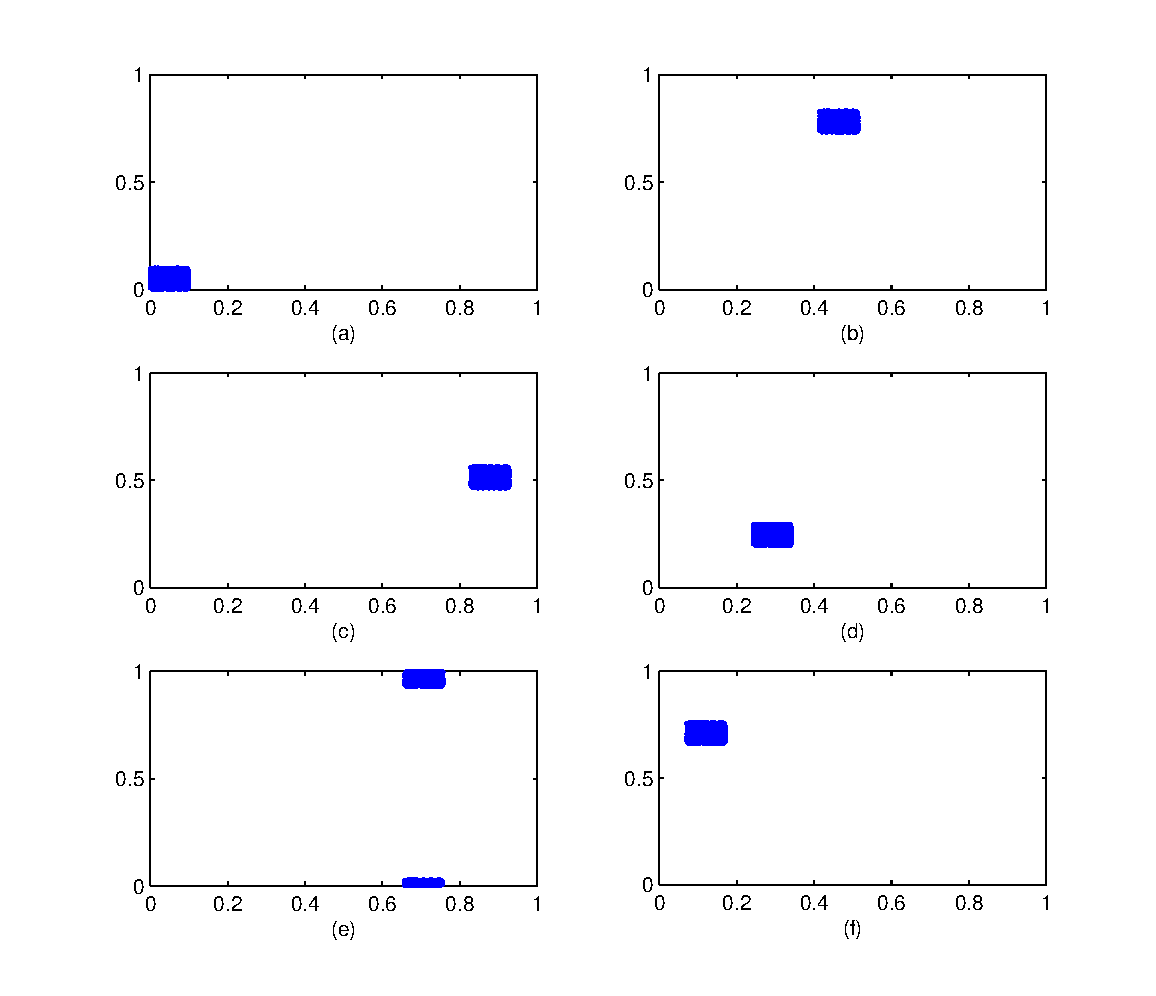
\includegraphics[width=.65\textwidth, height=1\textwidth,scale=0.5]{graficas/erg}
    \end{center}
    \caption{Iteraciones sucesivas de la transformaci�n \ref{t.erg}. Note como se mueve la distribuci�n de puntos en forma de cudrado sobre el espacio}

\end{figure}

\begin{figure}
    \begin{center}
        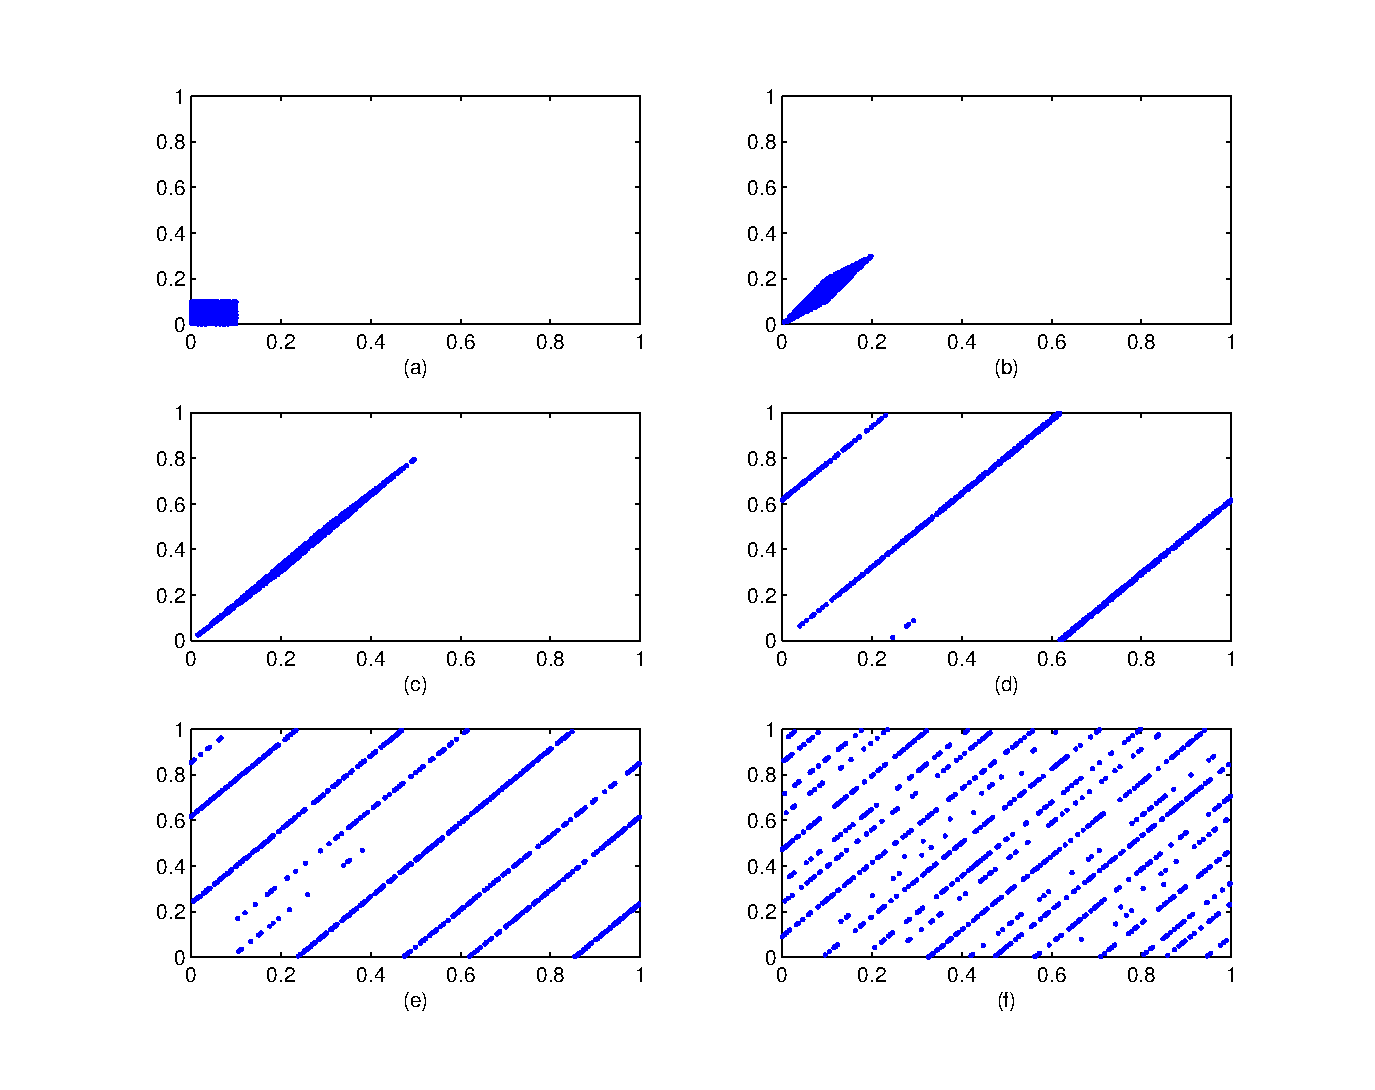
\includegraphics[width=.65\textwidth, height=1\textwidth,scale=0.5]{graficas/mix}
    \end{center}
    \caption{Iteraciones sucesivas de la transformaci�n \ref{t.mez}. Note como se esparce la distribuci�n de puntos sobre el espacio}

\end{figure}


\begin{figure}
    \begin{center}
        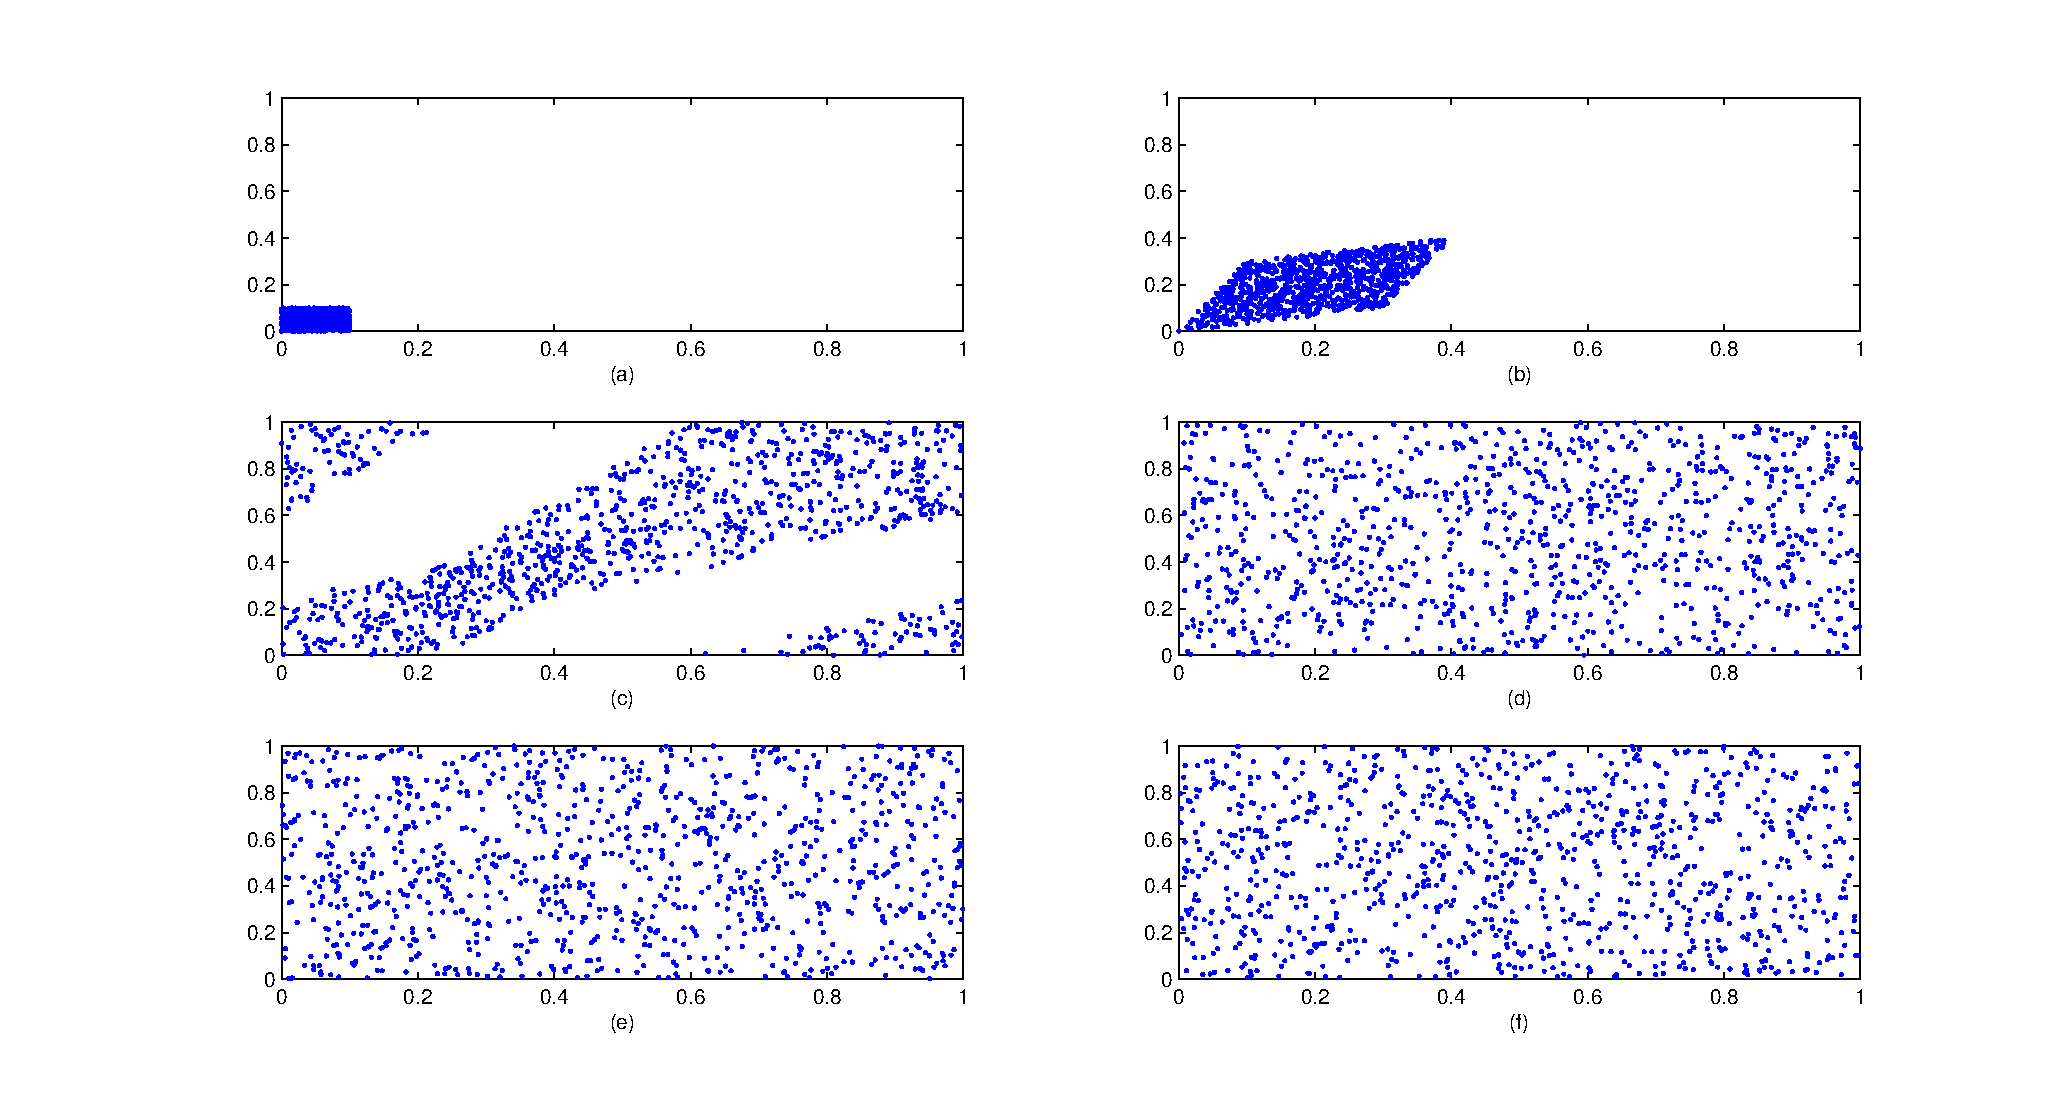
\includegraphics[width=.65\textwidth, height=1\textwidth,scale=0.5]{graficas/exa}
   \end{center}
    \caption{Iteraciones sucesivas de la transformaci�n \ref{t.exa}. Note como se esparce la distribuci�n de puntos sobre el espacio}

\end{figure}

\section{Taxonom�a de las Transformaciones}

Los conceptos desarrollados en las secciones previas para clasificar varios niveles de irregularidad en el comportamiento
est�n escritos en t�rminos de comportamiento de sucesiones de conjuntos. La pruebas de ergodicidad, mezclante o exacta
usando las definiciones son dif�ciles. En efecto los ejemplos presentados hasta ahora ilustran estos conceptos, no son rigurosas pruebas.

En esta secci�n se reformular� los conceptos de ergodicidad, mezclante y exacta en t�rmino del comportamiento de
sucesiones de iteraciones de los operadores de Perron-Forbenius y Koopman. Para mostrar c�mo pueden ser usadas para
determinar si una transformaci�n $S$ junto con una medida invariante es erg�dica, mezclante o exacta. Se requerir�
nociones sobre convergencia Cesaro, D�bil y Fuerte.

\begin{teo}Sea $(\X,\A,\R)$ una espacio de medida, $S:\X\cir$ una medida que preserva la transformaci�n y P el
    operador de Perron-Frobenius correspondiente a S. Entonces:
    \begin{description}
        \item[La transfomaci�n $S$ es erg�dica] si y solo si la sucesi�n converge Cesaro a 1 para todo $f\in D$.
        \item[La transfomaci�n $S$ es mezclante] si y solo si la sucesi�n converge d�bilmente a 1 para todo $f\in D$.
        \item[La transfomaci�n $S$  es exacto] si y solo si la sucesi�n converge fuertemente  a 1 para todo $f\in D$.
    \end{description}
\end{teo}

\subparagraph{Observaci�n} Note que como el operador $\Pm$ es lineal, la convergencia de la sucesi�n $\{\Pm^n f\}$ a 1 para
    $f\in D$ es equivalente a la convergencia de $\{\Pm^n f\}$ a $<f,1>$ para cada $f\in L^1$. Esta observaci�n es
    validad para todos los tipos de convergencia: Cesaro, D�bil, Fuerte. Por lo tanto,se reescribe el teorema.

\begin{teo}Sea $(\X,\A,\R)$ una espacio de medida, $S:\X\cir$ una medida que preserva la transformaci�n y $\Pm$
    el operador de Perron-Frobenius correspondiente a S. Entonces:
    \begin{description}
        \item[La transfomaci�n $S$ es erg�dica] si y solo si
        $$\limi_{n\rightarrow\infty}{\frac{1}{n}\sum_{k=0}^{n-1}{<\Pm^k f,g>=<f,1><1,g>}}\qquad f\in L^1,g\in L^\infty$$
        \item[La transfomaci�n $S$ es mezclante] si y solo si
        $$\limi_{n\rightarrow\infty}{<\Pm^k f,g>=<f,1><1,g>}\qquad f\in L^1,g\in L^\infty$$
        \item[La transfomaci�n $S$  es exacto] si y solo si
        $$\limi_{n\rightarrow\infty}{||\Pm^k f -<f,1>||>=0}\qquad f\in L^1$$
    \end{description}
\end{teo}

\begin{proof} Se probar� unicamente la condici�n de mezclante. Se asume la condici�n de
transformaci�n $S$ mezclante entonces por definici�n
\begin{align*}
    \limi_{n\rightarrow\infty}\mu(A\cap S^{B})&=\mu(A)\mu(B)  \\
\intertext{Reescribiendola en su forma integral}
    \limi_{n\rightarrow\infty}\int_\X\car_A(x)\car_B(x)(S^n(x))\mu(dx)&=\int_X\car_A(x)\mu(dx)\int_X\car_B(x)\mu(dx)\\
\intertext{Aplicando la definici�n del operador de Koopman}
    \limi_{n\rightarrow\infty}\int_\X\car_A(x)U^n\car_B(x)\mu(dx)&=\int_X\car_A(x)\mu(dx)\int_X\car_B(x)\mu(dx)\\
\intertext{Aplicando la defunci�n de producto escalar}
    \limi_{n\rightarrow\infty}<\car_A,U^n\car_B>&=<\car_A,1><1,\car_B>\\
\intertext{Usando la propiedad \eqref{c2n3} el operador de Perron-Frobenius es adjunto del operador de Koopman}
    \limi_{n\rightarrow\infty}<\Pm^n \car_A,\car_B>&=<\car_A,1><1,\car_B>\\
\intertext{Con lo que queda demostrado para $f=\car_A$ y $g=\car_B$.}
\end{align*}

Supongamos que $\tilde{A}=\cup_{i=1}^n{A_i}$, $\tilde{B}=\cup_{j=1}^m{B_j}$ y $\nu(A_i)=\lambda_k\delta_{ki}\mu(A_i)$
donde $\delta_{ik}$ es la delta de kronecker. N�tese que $\nu$ define una medida; supongase que S es mezclante, en consecuencia.

\begin{align*}
    \limi_{n\rightarrow\infty}\nu(\tilde{A}\cap S^{-1}(\tilde{B}))
     &=\limi_{n\rightarrow\infty}\nu(\cup_{i=1}^l{A_i}\cap S^{-1}(\cup_{j=1}^m{B_j})) \\
\intertext{Sustituyendo la definici�n de $\nu$}
     &=\limi_{n\rightarrow\infty}\lambda_h\delta_{hi}\lambda_k\delta_{kj}\sum_{i=1}^l{\sum_{j=1}^m{\mu(A_i\cap S^{-1}(B_j))}} \\
\intertext{Propiedades de la medida}
     &=\limi_{n\rightarrow\infty}\sum_{i=1}^l{\sum_{j=1}^m{\lambda_h\delta_{hi}\lambda_k\delta_{kj}\mu(A_i\cap S{-1}(B_j))}}\\
\intertext{Por linealidad}
     &=\limi_{n\rightarrow\infty}\sum_{i=1}^l{\sum_{j=1}^m{\lambda_i\lambda_j\mu(A_i\cap S{-1}(B_j))}} \\
\intertext{Evaluando las deltas de kronecker}
     &=\limi_{n\rightarrow\infty}\sum_{i=1}^l{\sum_{j=1}^m{\lambda_i\lambda_j\int_X{\car_{A_i}(x)\car_{B_j}(x)(S^n(x))\mu(dx)}}}\\
     &=\limi_{n\rightarrow\infty}\int_\X{\sum_{i=1}^l{\car_{A_i}(x)}\sum_{j=1}^m{U^n \car_{B_j}(x)\mu(dx)}}\\
     &=\limi_{n\rightarrow\infty}<\sum_{i=1}^l{\lambda_i\car_{A_i}(x)},\sum_{j=1}^m{U^n\lambda_j \car_{B_j}(x)}>\\
     &=\limi_{n\rightarrow\infty}<\sum_{i=1}^l{\Pm^n\lambda_i\car_{A_i}(x)},\sum_{j=1}^m{\lambda_j\car_{B_j}(x)}>\\
\intertext{Por otro lado, como $\nu$ es mezclante se tiene}
 \nu(A)\nu(B)&=\nu(\cup_{i=1}^l{A_i})\nu(\cup_{j=1}^m{B_j})  \\
             &=\lambda_h\delta_{hi}\sum_{i=1}^l{\mu(A_i)}\lambda_k\delta_{kj}\sum_{j=1}^m{\mu(B_j)}\\
             &=\sum_{i=1}^l{\lambda_i\mu(A_i)}\sum_{j=1}^m{\lambda_j\mu(B_j)}\\
             &=\sum_{i=1}^l{\lambda_i\int_\X\car_A(x)\mu(dx)}\sum_{j=1}^m{\lambda_j\int_X{\car_B(x)\mu(dx)}}\\
             &=\int_\X{\sum_{i=1}^l{\lambda_i\car_A(x)\mu(dx)}}\int_\X{\sum_{j=1}^m{\lambda_j\car_B(x)\mu(dx)}}\\
             &=<\sum_{i=1}^l{\lambda_i\car_{A_i}},1><1,\sum_{j=1}^m{\lambda_j\car_{B_i}}>
\end{align*}
Y por lo tanto se cumple para funciones simples. Adicionalmente, para cada $g\in L\infty$ es convergente a un limite de funciones simples en 
$g_k\in\infty$ y para cada funci�n $f\in L^1$ tiene convergencia fuertemente a la sucesi�n de funciones simples $f_h\in L^1$. Se tiene la siguiente relaci�n
\begin{align*}
|<\Pm^n f, g>-<f,1><1,g>|&\leq|<\Pm f,g>-<\Pm^n f_k,g_k>|\\
                         &+|<\Pm^n f_k,g_k>-<f_k,1><1,g_k>|\\
                         &+|<f_k,1><1,g_k>-<f,1><1,g>|   
\end{align*}  

Si $||f_k-f||\leq\epsilon$ y $||g_k-g||\leq\epsilon$ entonces se satisface 
\begin{align*}
|<\Pm f,g>-<\Pm^n f_k,g_k>|&\leq|<\Pm^n f,g>-<\Pm^n f_k,g>|\\
                           &+|<\Pm^n f_k,g>-<\Pm^n f_k,g_k>|\\
                           &\leq\epsilon ||g||_{L^\infty}+\epsilon||f_k||\\
                           &\leq\epsilon(||g||_{L^\infty}+||f||+\epsilon)
\end{align*}

Se forma analoga se prueba 

$$|<f_k,1><1,g_k>-<f,1><1,g>|\leq\epsilon(||g||_{L\infty}+||f||+\epsilon)$$

Como estos t�rminos son arbitrariamente peque�os para $\epsilon$. Finalmente, el t�rmino

$$|<\Pm^n f_k,g_k>-<f_k,1><1,g_k>|$$ 

Converge a cero para $n\rightarrow\infty$. Esto completa la prueba de que es mezclante implica $<\Pm^n f,g>$ a $<f,1><1,g>$ para todo 
$f\in L^1$ y $g\in L^\infty$. La implicaci�n opuesta se demuestra tomando el conjunto $f=\car_A$ y $g=\car_B$.

\end{proof}




